\documentclass{article}
\usepackage[spanish]{babel}   
\usepackage[numbers,sort&compress]{natbib}
\usepackage{float}
\usepackage{listings}
\usepackage{graphicx} 	% Nos permite importar imagenes 
\usepackage{subcaption}
\usepackage[left=3cm,right=3cm,top=3cm,bottom=3cm]{geometry}

%-------------------------- Por si se romple la URL --------------------------
\usepackage[hyphens]{url}
\usepackage[hidelinks]{hyperref}
\hypersetup{breaklinks=true}	
\urlstyle{same}
\usepackage{cite}
%-------------------------- Por si se romple la URL --------------------------

\title{Reporte Tarea 4}
\author{Victor Alejandro Oviedo Martínez}



\begin{document}
\maketitle
\hrule

\section{Introduccón}\label{intro}
Para esta cuarta tarea\citep{DRA.P4} se ha estudiado el tema Diagramas de Voronoi, para esta tarea solo será representado en dos dimensiones, por lo tanto, se tendrá un plano que en este caso será un plano cuadrado. Una vez determinado el plano se asignan puntos a los cuales llamaremos semillas, estas semillas son distribuidas aleatoriamente para después delimitar el espacio entre ellas. Para delimitar el espacio entre ellas se lleva a cabo una acción repetitiva, en la cual se toman dos diferentes puntos y se mide la distancia euclidiana entre ellos, una vez determinada la distancia se traza una linea perpendicular a la mitad de la medición, con esto estaremos delimitando el área entre estos dos puntos y tendremos que el área siempre pertenecerá a la semilla mas cercana. Este proceso será repetido para cada semilla en el plano con todas las semillas vecinas. Al final de este proceso tendremos un conjunto de celdas las cuales tendrán una área determinada por la distancia entre ella y sus vecinas. Ahora podemos decir que tenemos completo un diagrama Voronoi, sin embargo, dado el parecido del diagrama Voronoi con las estructuras formadas por algunos materiales, este se utiliza para la simulación de microfracturas. Por lo que a este diagrama de Voronoi se le agrega la simulación de  una fractura, tomando en cuenta que esta fractura tendrá una posición inicial asignada aleatoriamente. Esta fractura podrá avanzar tomando en cuenta dos porcentajes, el porcentaje entre celdas y porcentaje dentro de la celda. La fractura podrá avanzar hasta que ya no tenga hacia dónde avanzar, o que el porcentaje dentro de celda sea cero.\\


 

\section{Desarrollo}

Para esta cuarta tarea se ha planteado el siguiente problema: Examina de manera sistemática el efecto del número de semillas y del tamaño de la zona en la distribución en las grietas que se forman en términos o (1) la mayor distancia euclideana entre la grieta y el exterior de la pieza o (2) sí o no parte la pieza.\\

Para el desarrollo de esta tarea se a utilizado el código ejemplo proporcionado por la Dra. \citet{DRA.Code}, tiene el propósito de desarrollar una diagrama de Voronoi, el cual será utilizado para el estudio del largo de múltiples fracturas probadas en el mismo diagrama. Esté código será  tomando como base y modificando para las características de esta tarea.\\

En este caso se eligió la opción (1), por lo tanto, se inicio pensando una forma en la cual se pueda medir de forma correcta la mayor distancia euclideana entre la grieta y el exterior. A esto surgió la idea de la obtención de la mayor distancia por medio de cuadrantes, en el cual a nuestro plano se divide en 4 partes iguales por medio de dos lineas las cuales son perpendicular y convergen en el centro del plano. Esto se hizo, para dependiendo la posición en la  que esté la parte de la fractura evaluada, se le asigne punto de referencia  para la medición. Esto se agregó dentro de la función \texttt{propagar(replicar)}, de este modo al momento de generar fractura también se mida su distancia. \\

\begin{lstlisting}[language=Python]
        if x < mitad and y < mitad:
            xout = 0
            yout = 0
            dist = sqrt(((x - xout) **2) + ((y - yout)**2))
        elif x > mitad and y < mitad:
            xout = n
            yout = 0
            dist = sqrt(((xout - x)**2) + ((yout + y)**2))
        elif x < mitad and y > mitad:
            xout = 0
            yout = n
            dist = sqrt(((xout + x)**2) + ((yout - y)**2))
        elif x > mitad and y > mitad:
            xout = n
            yout = n
            dist = sqrt(((xout - x)**2) + ((yout - y)**2))

        if dist > mindist:
            mindist = dist
            maxdist= dist
            
 \end{lstlisting}
 
Como se pude ver en la parte superior, se tiene la parte del código en la cual se selecciona el cuadrante perteneciente, para esto se utiliza la posición de la fractura actual representada por \texttt{x}, \texttt{y}, estas son comparadas con la variable \texttt{mitad} la cual representa la mitad de nuestro plano, al ser nuestro plano cuadrado esta función sirve tanto para el eje X, como para el eje Y. Una vez seleccionado el cuadrante se la asigna el punto de referencia y se calcula su distancia. Por último, se compara si la distancia actual es la mas larga, una vez que la fractura no pueda avanzar más la función \texttt{propagar(replicar)} regresará  la distancia máxima de toda la fractura.\\

Una vez que la función \texttt{propagar(replicar)} entrega valores correctos, se procedió ha agregar el código necesario para evaluar fracturas con diferente tamaño de plano \texttt{(N)} y diferente cantidad de semillas \texttt{(k)}, sin embargo en este caso utilizaremos un coeficiente \texttt{(K)} para determinar la cantidad de semillas \texttt{(k)}, esto con la finalidad de visualizar un efecto independiente de la escala. Por lo tanto, se tendrá la cantidad de semillas \texttt{(k)} dependiendo del tamaño del plano \texttt{(N)}, esto es igual a \texttt{k = K × N}.    


\begin{lstlisting}[language=Python]
N = [50, 100, 150, 200]
K = [1, 2, 4, 8, 16, 32]
gg = []
for n in N:
    print("------------------",n ,"------------------")
    gg = []
    for o in K:
        print("------------------",n,o,"------------------")
        semillas = []
        k = n * o
        for s in range(k):
            while True:
                x, y = randint(0, n - 1), randint(0, n - 1)
                if (x, y) not in semillas:
                    semillas.append((x, y))
                    break
 \end{lstlisting}


Por último, todos los datos son guardados y gráficados. Para el desarrollo de esta tarea se utilizó la pagina \citep{DRA.Code}.


\section{Conclusión}

Como se pude observar en la Figura \ref{fig:cuadro.1} se he realizado la simulación de grietas en diagrama Voronoi para cuatro diferentes tamaños de plano, seis diferentes coeficientes de semillas, y cien iteraciones para cada combinación.   



\begin{figure}[H]
\begin{center}
	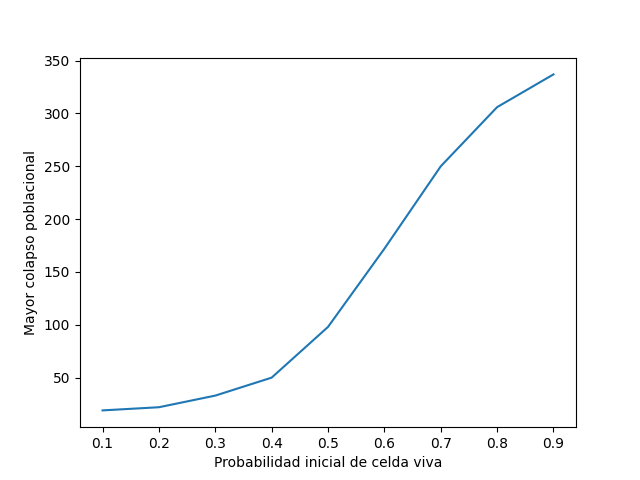
\includegraphics[height=2.65in]{/Users/victor/Desktop/Figure_1.png}
	\caption{ Resultados de la simulación a 100 repeticiones (coeficiente de semillas).}
	\label{fig:cuadro.1}
\end{center}
\end{figure}


Dado que en la Figura \ref{fig:cuadro.1} no refleja los resultados esperados, se procedió a realizar la misma prueba sin embargo esta vez con cantidades específicas de semillas a lo que nos da como resultado la figura  \ref{fig:cuadro.2}

\begin{figure}[H]
\begin{center}
	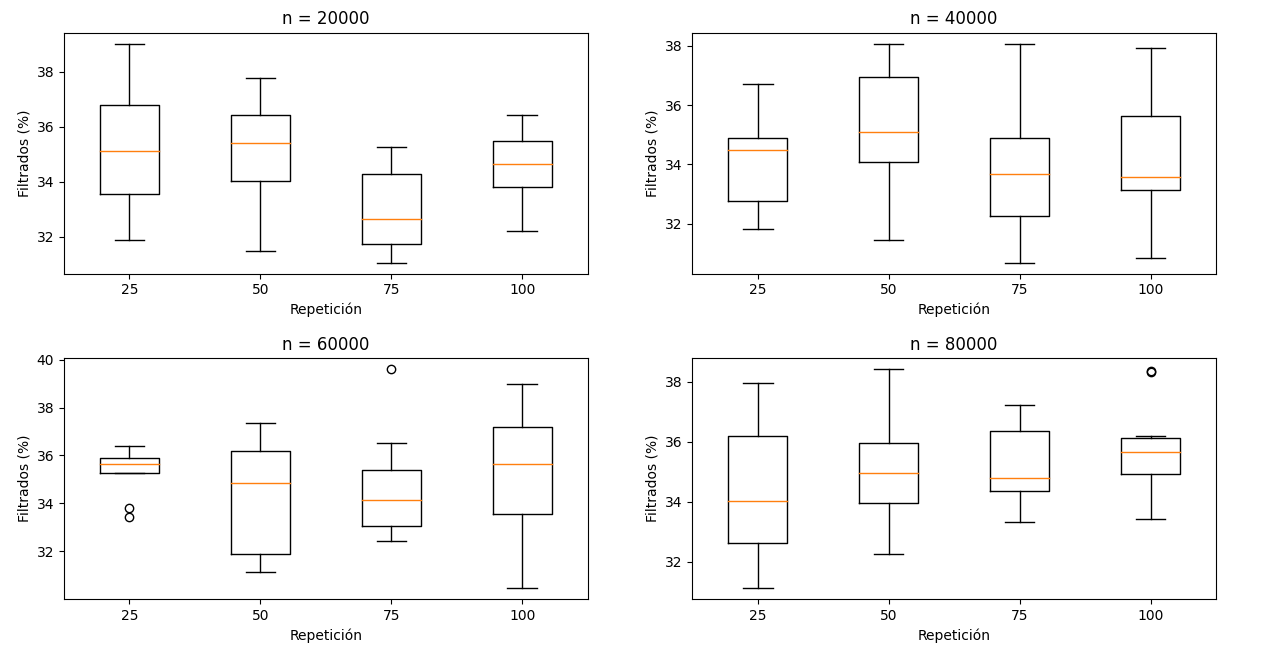
\includegraphics[height=2.65in]{/Users/victor/Desktop/Figure_2.png}
	\caption{ Resultados de la simulación a 100 repeticiones (cantidad de semillas).}
	\label{fig:cuadro.2}
\end{center}
\end{figure}
Comparando los valores de la Figura \ref{fig:cuadro.1}  con la Figura \ref{fig:cuadro.2} se pudo razonar que los resultados de las figuras son resultados correctos. Ya que no importa la cantidad de semillas, ni el tamaño del diagrama, para obtener mayor o menor distancia entre la grieta y el exterior de la pieza, ya que lo que real mente importa es la posición inicial de la grieta y la distancia que se pueda mover al centro de la pieza.

%-------------------------- Por si se rompe la URL --------------------------
\Urlmuskip=0mu plus 1mu\relax
%-------------------------- Por si se rompe la URL --------------------------
\bibliography{ref.Tarea4.bib}
\bibliographystyle{plainnat}

\end{document}